\documentclass[fleqn,a4paper,11pt]{report}
\usepackage[italian]{babel}
\usepackage[margin=1in]{geometry}
\usepackage[final]{graphicx}
\usepackage{amsmath}
\usepackage{amsthm}
\usepackage{wasysym}
\usepackage{stmaryrd}
\usepackage{amsfonts}
\usepackage[utf8x]{inputenc}
\usepackage{booktabs}
\usepackage{url}
\usepackage{listings}
\lstset{mathescape,columns=fullflexible,basicstyle=\fontfamily{lmvtt}\selectfont}
\usepackage{caption} 
\setlength\abovecaptionskip{.4em}
\setlength\belowcaptionskip{.8em}
\usepackage{hyperref}
\usepackage{titlesec}  


%\usepackage{titlesec}
%\titleformat*{\section}{\Huge\bfseries}

\usepackage{tikz}
\usetikzlibrary{calc}
\newcommand\HRule{\rule{\textwidth}{1pt}}
\newcommand\LRule{\rule{\textwidth}{.5pt}}
\newcommand\DRule{\rule{\textwidth}{.4pt}\\[\dimexpr-\baselineskip+1mm+2pt] \rule{\textwidth}{2pt}}

\usepackage{titlesec}
\titleformat{\chapter}[hang]
{\normalfont\huge\bfseries}{\chaptertitlename\ \thechapter:}{.3em}{} 

%\titlespacing*{<command>}{<left>}{<before-sep>}{<after-sep>}
\titlespacing*{\chapter}
{0pt}{5.5ex plus 1ex minus .2ex}{3.3ex plus .2ex}

\begin{document}

% begin intro
\begin{titlepage}
\begin{center}
	\begin{minipage}{6in}
  		\centering
  		\raisebox{-0.5\height}{
\includegraphics[height=80px]{img/pollo.png}}
  		\hspace*{1.6in}
  		\raisebox{-0.5\height}{
\includegraphics[height=20px]{img/logoDM.png}}
  		%\hspace*{.35in}
	\end{minipage}\\[.5cm]
% Upper part of the page
\textsc{\LARGE Universit\`a di Padova}\\[.2cm]
\textsc{\large Dipartimento di Matematica\\
			Corso di Laurea Magistrale in Informatica}\\[.3cm]
\DRule \\[.5cm]
% Title
{ \huge \bfseries Corso di Intelligenza Artificiale}\\[.4cm]
{\Large Marco Romanelli, [1106706]} \\[1cm]
{\large \today}
\HRule \\[3cm]
\end{center}
\end{titlepage}
\newpage
% end intro

%%%%%%%%%%%%
% begin document
\chapter{Introduzione}
\section{Fase iniziale}
La fase iniziale del progetto consiste in una prima analisi delle principali piattaforme che offrono servizi di \textit{Cognitive Computing}, considerando vantaggi e svantaggi di ognuna.
Data la diversificazioni di proposte all'intero di ogni piattaforma, per l'analisi e la comparazione ci siamo focalizzati sul riconoscimento di immagini.


%%%%%%%%%%%%
\section*{}
Procederemo nel seguente modo: nel Capitolo 2 verrà presentata una panoramica dei servivi presi in esame e seguirà poi nel Capitolo 3 l'analisi dettagliata per ogni servizio.
Il Capitolo 4 contiene una sintesi sulle tariffe richieste per ogni servizio.
Il Capitolo 5 riassume le conclusioni della squadra di lavoro. 
Il capitolo 6 concluderà con alcuni possibili sviluppi di questa analisi.

\section{Snippet}
In un'analisi è spesso necessario anche definire un possibile caso d'uso (obbietto) ed effettuare delle prove in relazione a tale contesto. Questo sia per approfondire l'analisi in sé e sia per poter comparare le diverse soluzioni offerte in un contesto reale (anche se limitato).

Si immagini, quindi, di dover analizzare degli scontrini fiscali con l'obbiettivo di informatizzare le informazioni contenutevi, come ad esempio il locale che ha emesso lo scontrino, le voci con i relativi prezzi, il giorno di emissione, eccetera.
Questo perché, ad esempio, un'azienda potrebbe aver bisogno di un sistema che permetta l'analisi degli scontrini per stabilire se e in che misura attribuire dei rimborsi ai propri dipendenti.

Per ogni soluzione si effettueranno alcune prove in relazione al contesto appena descritto, analizzandone pregi e difetti, tenendo ovviamente in considerazione la natura limitata delle stesse.


%%%%%%%%%%%%
{\let\clearpage\relax \chapter{Cognitive Computing}}
\section{Introduzione}
% TODO


\section{Servizi disponibili}
Le maggiori piattaforme per il \textit{Cognitive Computing} sono offerte da alcune fra le maggiori aziende nell'ambito informatico e tecnologico e sono:
\begin{itemize}
\item Microsoft Cognitive Services\cite{mcs-link} (Microsoft Corporation),
\item Watson Developer Cloud (IBM: International Business Machines Corporation),
\item Amazon Artificial Intelligence (Amazon.com, Inc)
\item Google Cloud Platform (Google Inc.)
\end{itemize}



%%%%%%%%%%%%
{\let\clearpage\relax \chapter{Analisi dei servizi}}
\section{Microsoft Cognitive Services: Computer Vision API}
\subsection{Panoramica}
\paragraph{Prerequisiti}
\begin{itemize}
\item Input: dati grezzi (stream application/octet) o url;
\item Formati supportati: JPEG, PNG, GIF, BMP;
\item Dimensione file massima: 4 MB;
\item Dimensione immagine minima: 50x50 pixel. 
\end{itemize}
%

Le API\footnote{\url{https://www.microsoft.com/cognitive-services/en-us/computer-vision-api}} sono molteplici, a seconda dello scopo finale dell'analisi visiva.

\paragraph{Tagging} Le API ritornano un insieme di etichette (in formato JSON) che descrivono gli oggetti presenti nell'immagine, come oggetti, esseri viventi, azioni, paesaggi; per ogni etichetta viene anche fornito il livello di \textit{confidence} (affidabilità). I tag non sono in alcun modo organizzati fra loro e non esiste nessun tipo di ereditarietà.
Nel caso un tag sia ambiguo viene fornito in aggiunta un \textit{hint} che ne spiega il contenuto.
Al momento la sola lingua supportata è l'inglese.

\paragraph{Classificazione} L'immagine viene classificata in categorie che seguono una tassonomia con ereditarietà di tipo padre-figlio. Questa tassonomia prevede 86 categorie\footnote{\url{https://www.microsoft.com/cognitive-services/en-us/Computer-Vision-API/documentation/Category-Taxonomy}} e classifica gli elementi visivi in modo più o meno specifico.

\paragraph{Identificazione del tipo} E' possibile classificare l'immagine come in bianco o nero o a colori, se è un disegno o se è del tipo \textit{clip-art}; in quest'ultimo caso viene fornito un livello di qualità dell'immagine, compreso fra 0 e 3.

\paragraph{Riconoscimento volti} Riconosce i volti umani e restituisce la posizione (coordinate) di questi all'interno dell'immagine, come anche età e sesso della persona.

\paragraph{Contenuto personalizzato} Ideato per raffinare la tassonomia a 86 categorie utilizzando informazioni specifiche sul dominio. Attualmente è supportato solamente il riconoscimento dei volti delle persone famose.

\paragraph{Generazione di descrizioni} Genera una lista di frasi (in lingua inglese) che descrivono il contenuto dell'immagine, ordinate secondo un livello di affidabilità calcolato per ogni descrizione.

\paragraph{Estrazione colori} Identifica i colori analizzandoli in tre contesti: di sfondo, in primo piano e d'insieme; i colori sono raggruppati in 12 colori predominanti. Classifica le immagini fra in bianco e nero e a colori.

\paragraph{Riconoscimento contenuti non adatti ai minori} Riconosce materiali pornografici e contenuti osé in generale. Può essere impostato un livello per il filtro.

\paragraph{Riconoscimento del testo (OCR)} Rileva il testo presente nell'immagine e lo trasforma affinché sia leggibile da una macchina, ruota l'immagine se necessario per rendere il testo orizzontale e fornisce le coordinate per ogni parola. Al momento sono supportati 21 linguaggi, fra cui l'inglese, l'italiano, il francese, il tedesco e lo spagnolo.

L'accuratezza del riconoscimento dipende dalla qualità dell'immagine ed eventuali errori possono essere causati da immagini sfuocate, scrittura a mano, testo troppo piccolo, ecc.
   
\paragraph{Creazione anteprime} Un'anteprima è una rappresentazione dell'immagine in scala ridotta. L'immagine viene prima analizzata e poi ritagliata secondo la ``regione di interesse'' (ROI); il rapporto dell'immagine (\textit{aspect ratio}) può essere impostato secondo le proprie preferenze.


\subsection{Tariffe} Due tipologie di piani:
\begin{itemize}
\item Gratuito: fino a 5000 chiamate al mese, massimo 20 chiamate al minuto;
\item Standard: 0,015\$ a chiamata, fino a 10 TPS.
\end{itemize}


\subsection{Esecuzione}


\paragraph{} 

La prova è stata eseguita utilizzando la funzione OCR.
\begin{figure}[htbp]
\begin{center}
	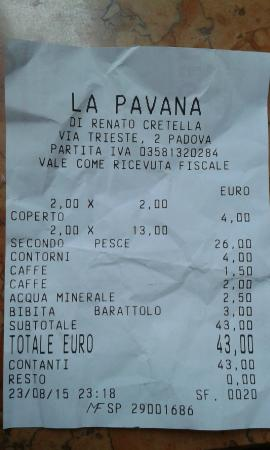
\includegraphics[height=.5\textwidth]{img/scontrino.jpg}
  	\hspace*{1in}
	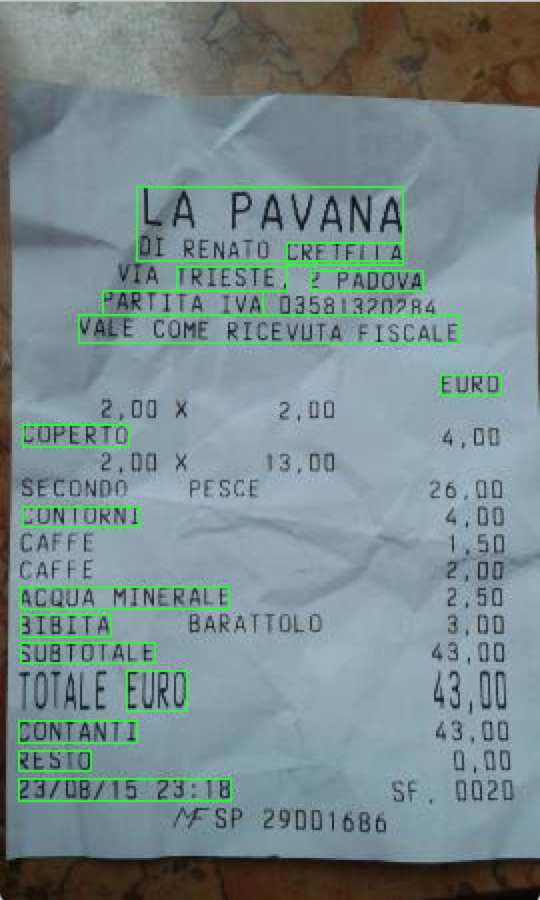
\includegraphics[height=.5\textwidth]{img/ms-ocr.png}
\caption{default}
\label{default}
\end{center}
\end{figure}


%%\subsection{Riassunto}


%%%%%%%%%%%%
%%{\let\clearpage\relax \bibliography{biblio.bib}}
\bibliography{biblio.bib}
\bibliographystyle{alpha} % oppure abbrv

%
% end document
\end{document}
